\section{全体構成}\label{ux5168ux4f53ux69cbux6210}

\subsection{概略}\label{ux6982ux7565}

機体の全体図をFig.\ref{fig15}に示します。

この機体は底部フレームを土台として、脚ユニットが4つ締結されています。
底部フレームは箱型形状をしており、内側にはバッテリーや制御回路などの電装系が内蔵されています。
この構成により、機体組立後は外側から電装系にアクセスできないようになっています。

中間フレームは底部フレームの天面に取り付けられ、蓋の役割も兼ねています。
中間フレームには2枚の側面フレームが締結され、左右のフレーム間にアームの全部品が取り付けられています。

脚部を駆動するギアドモータは各脚に1つずつ搭載されており、アームにも独立したモータが搭載されています。

次に機体の分解図をFig.\ref{fig16}に示します。

中間フレームは、底部フレームとネジ2本だけで締結されており、底部フレームと中間フレームは容易に組立・分解が可能です。
また、脚ユニットは4つ全て共通であるため、どの場所にでも取り付けることが可能です。

脚ユニットの取り付け方法ですが、底部フレームを挟み込んだ後に、ネジ1本のみで固定する構成としました。
故障時の交換対応がしやすくなっています。
これによりメンテナンス性の向上を狙っています。

\begin{figure}[htbp]
\centering
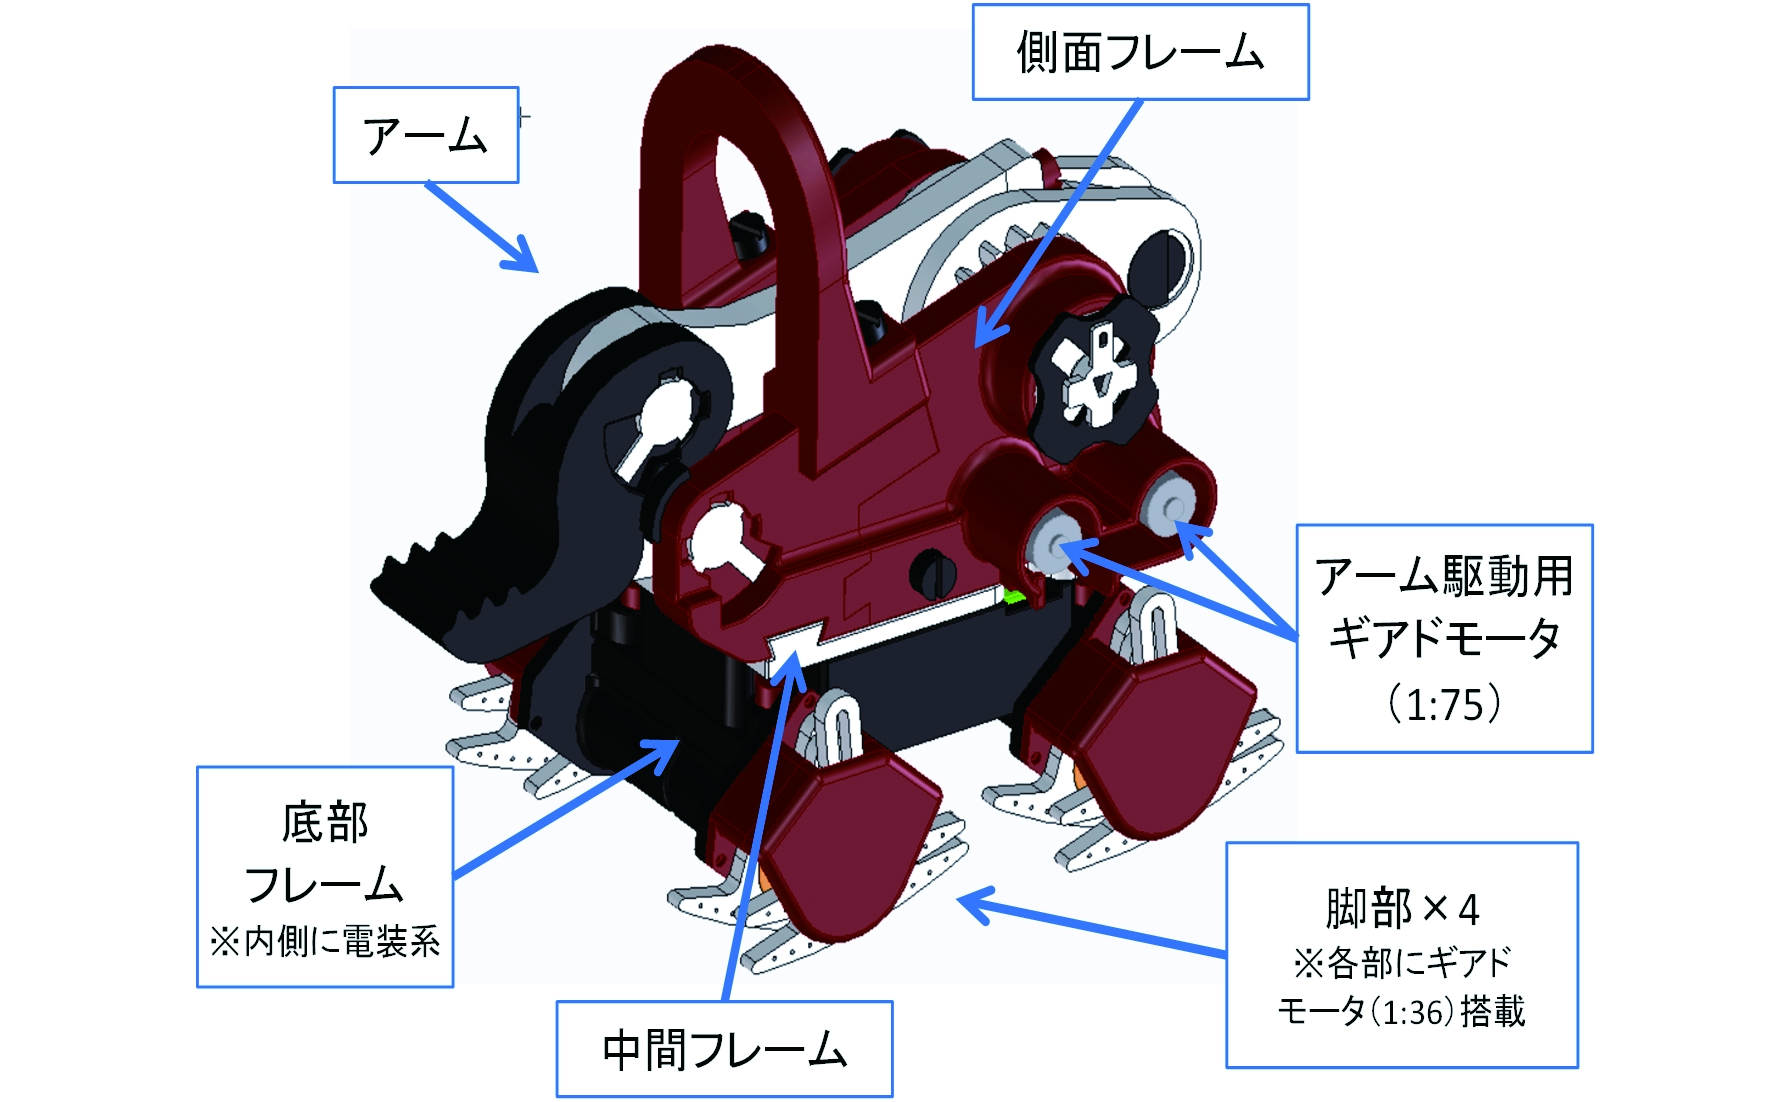
\includegraphics[width=400pt]{fig/fig15_cmyk.jpg}
\caption{機体の全体像}
\label{fig15}
\end{figure}

\begin{figure}[htbp]
\centering
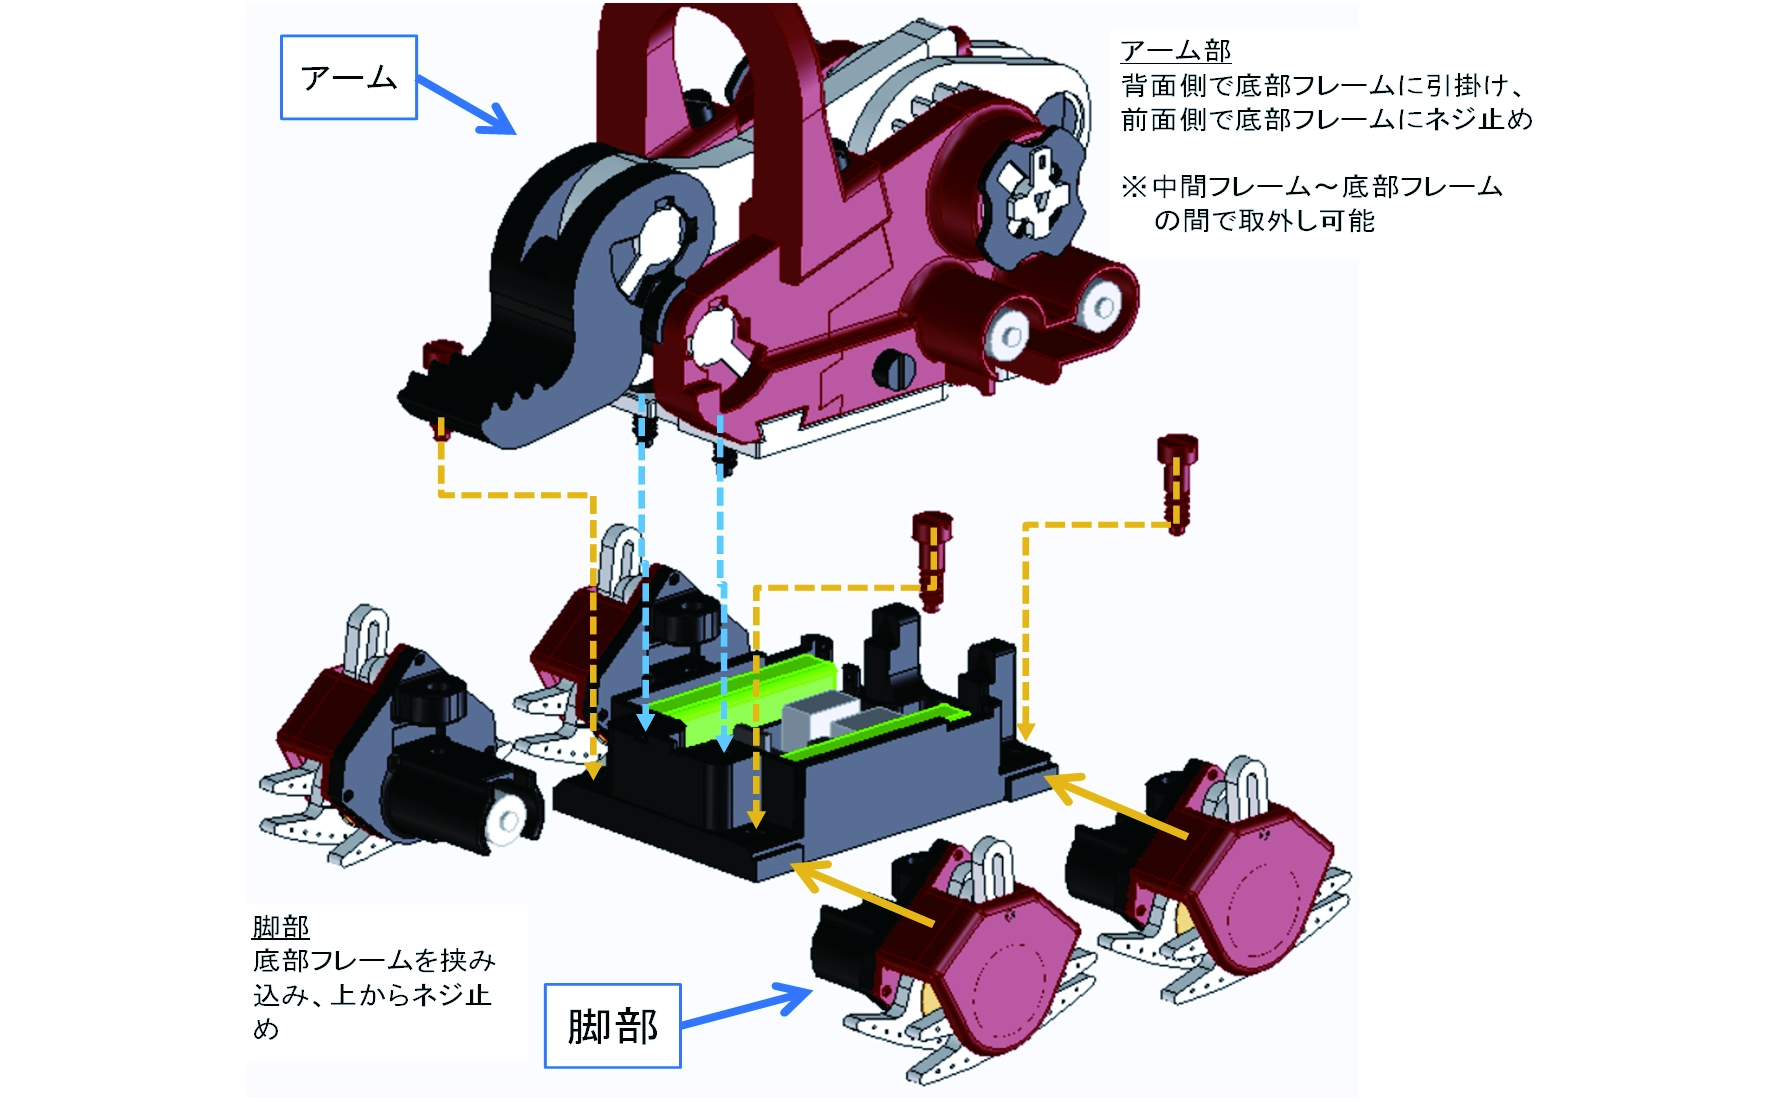
\includegraphics[width=400pt]{fig/fig16_cmyk.jpg}
\caption{機体の分解図}
\label{fig16}
\end{figure}

\clearpage

\subsection{機体の状態とサイズ}\label{ux6a5fux4f53ux306eux72b6ux614bux3068ux30b5ux30a4ux30ba}

機体の各状態とサイズの関係は下記の通りに設計しました。

\begin{itemize}
\tightlist
\item
  Fig.\ref{fig17}(a)
  停止状態。規格サイズに収まるようにアーム先端を分割し、アーム長を短くした状態で待機しています
\item
  Fig.\ref{fig17}(b)
  走行時の状態。開始直後にアームを動かすと、アーム先端が自重で回転しアーム長が伸びます
\item
  Fig.\ref{fig17}(c)
  相手機体攻撃時の状態を示した斜視図。基本設計で検討した通り射程距離は機体全面から250mmとなっています
\end{itemize}

\begin{figure}[htbp]
\centering
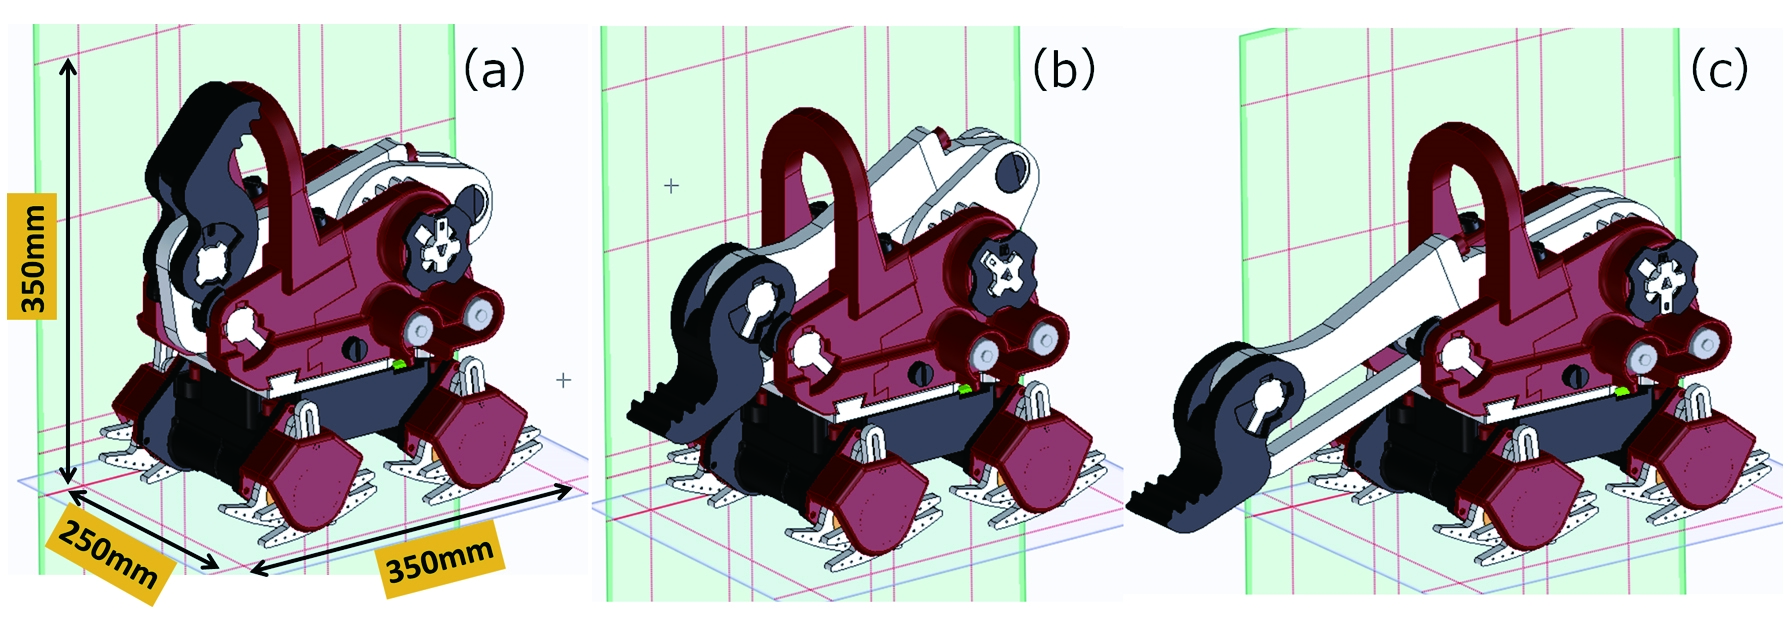
\includegraphics[width=380pt]{fig/fig17_cmyk.jpg}
\caption{機体の状態とサイズ}
\label{fig17}
\end{figure}

\section{アーム構成の詳細}\label{ux30a2ux30fcux30e0ux69cbux6210ux306eux8a73ux7d30}

アーム構成は第3章で決定したパラメータで設計を行った。
側面からみた断面図を Fig.\ref{fig18}に示します。

アーム駆動用ギアドモータ(1:75)は小ギアに接続されており、合計4つのギアドモータの駆動力がアームへと伝達されます。
駆動伝達経路は、ギアドモータ、小ギア、大ギア(第1クランクと接合されている)となっています。
小ギアと大ギアの減速比は第3章で計算した通り、1.6としています。

アームの第2クランクには相手機体攻撃時に大きな力が加わります。
こちらも第3章で計算した通り、幅32mm以上、厚み23mm以上を確保して設計しています。

実際に必要強度が確保されているかは不明ですが、試合時にアーム部の部品破損は発生しませんでした。
実用上は問題ないレベルで設計できていたのではないかと思います。

\begin{figure}[htbp]
\centering
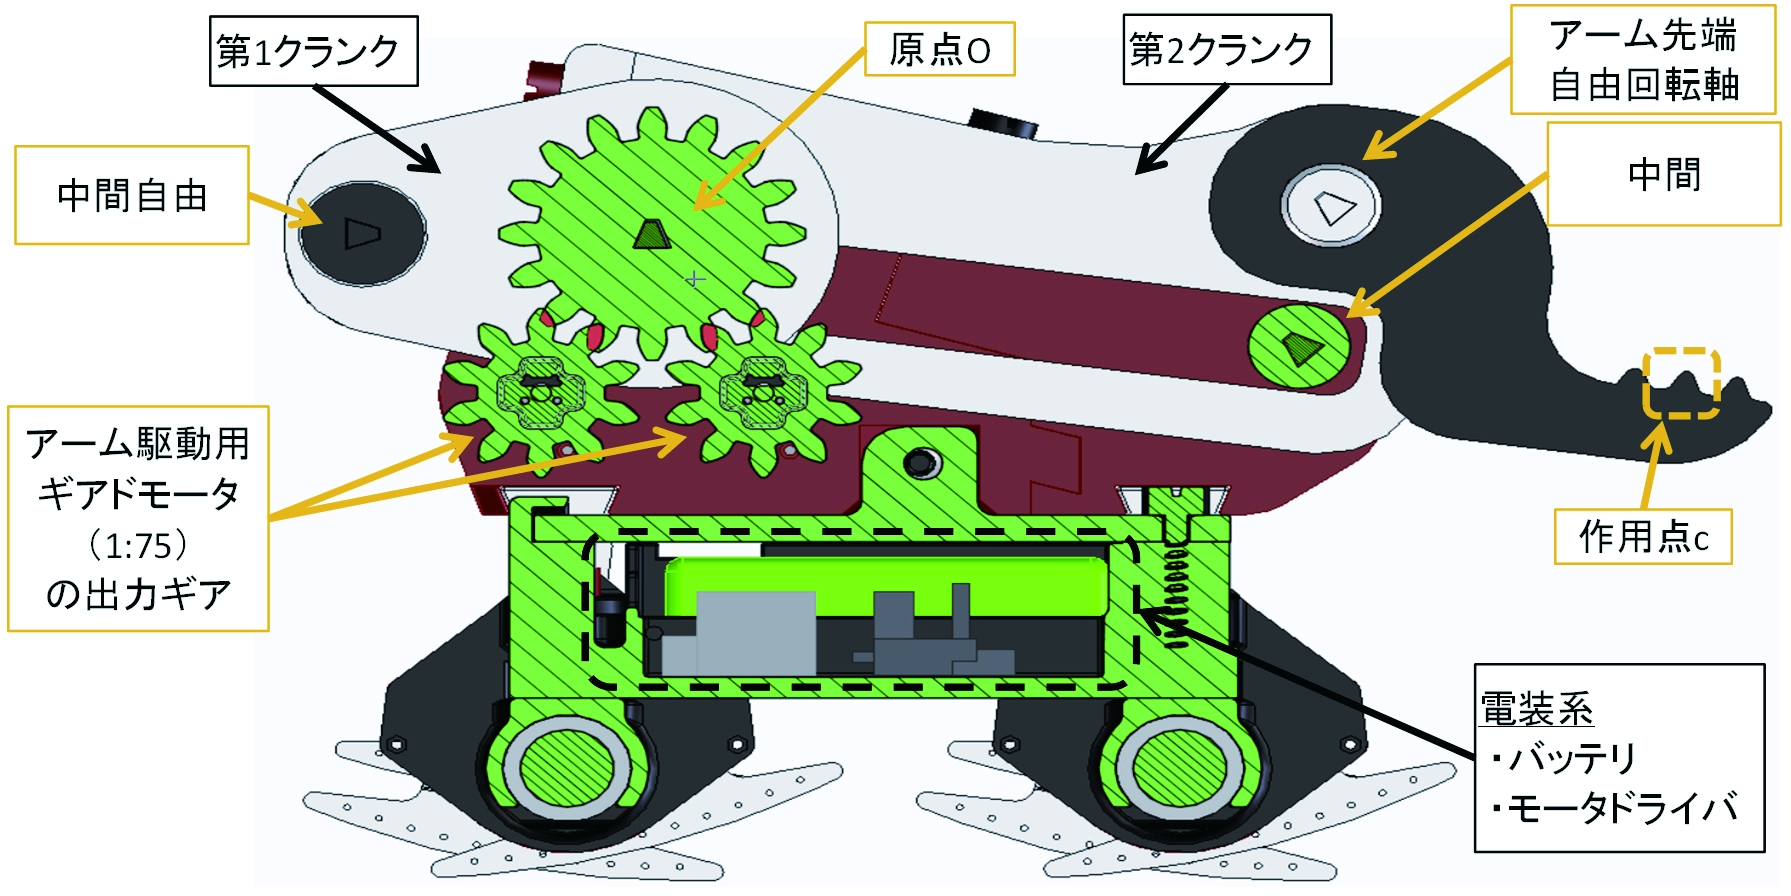
\includegraphics[width=380pt]{fig/fig18_cmyk.jpg}
\caption{アーム構成}
\label{fig18}
\end{figure}

\section{積層方向の割れ防止構成}\label{ux7a4dux5c64ux65b9ux5411ux306eux5272ux308cux9632ux6b62ux69cbux6210}

負荷がかかる部分に関しては積層方向の割れ防止構成を盛り込んで設計を行いました。
負荷のかかる箇所と実際の設計構成をFig.\ref{fig20}に示します。

\begin{figure}[htbp]
\centering
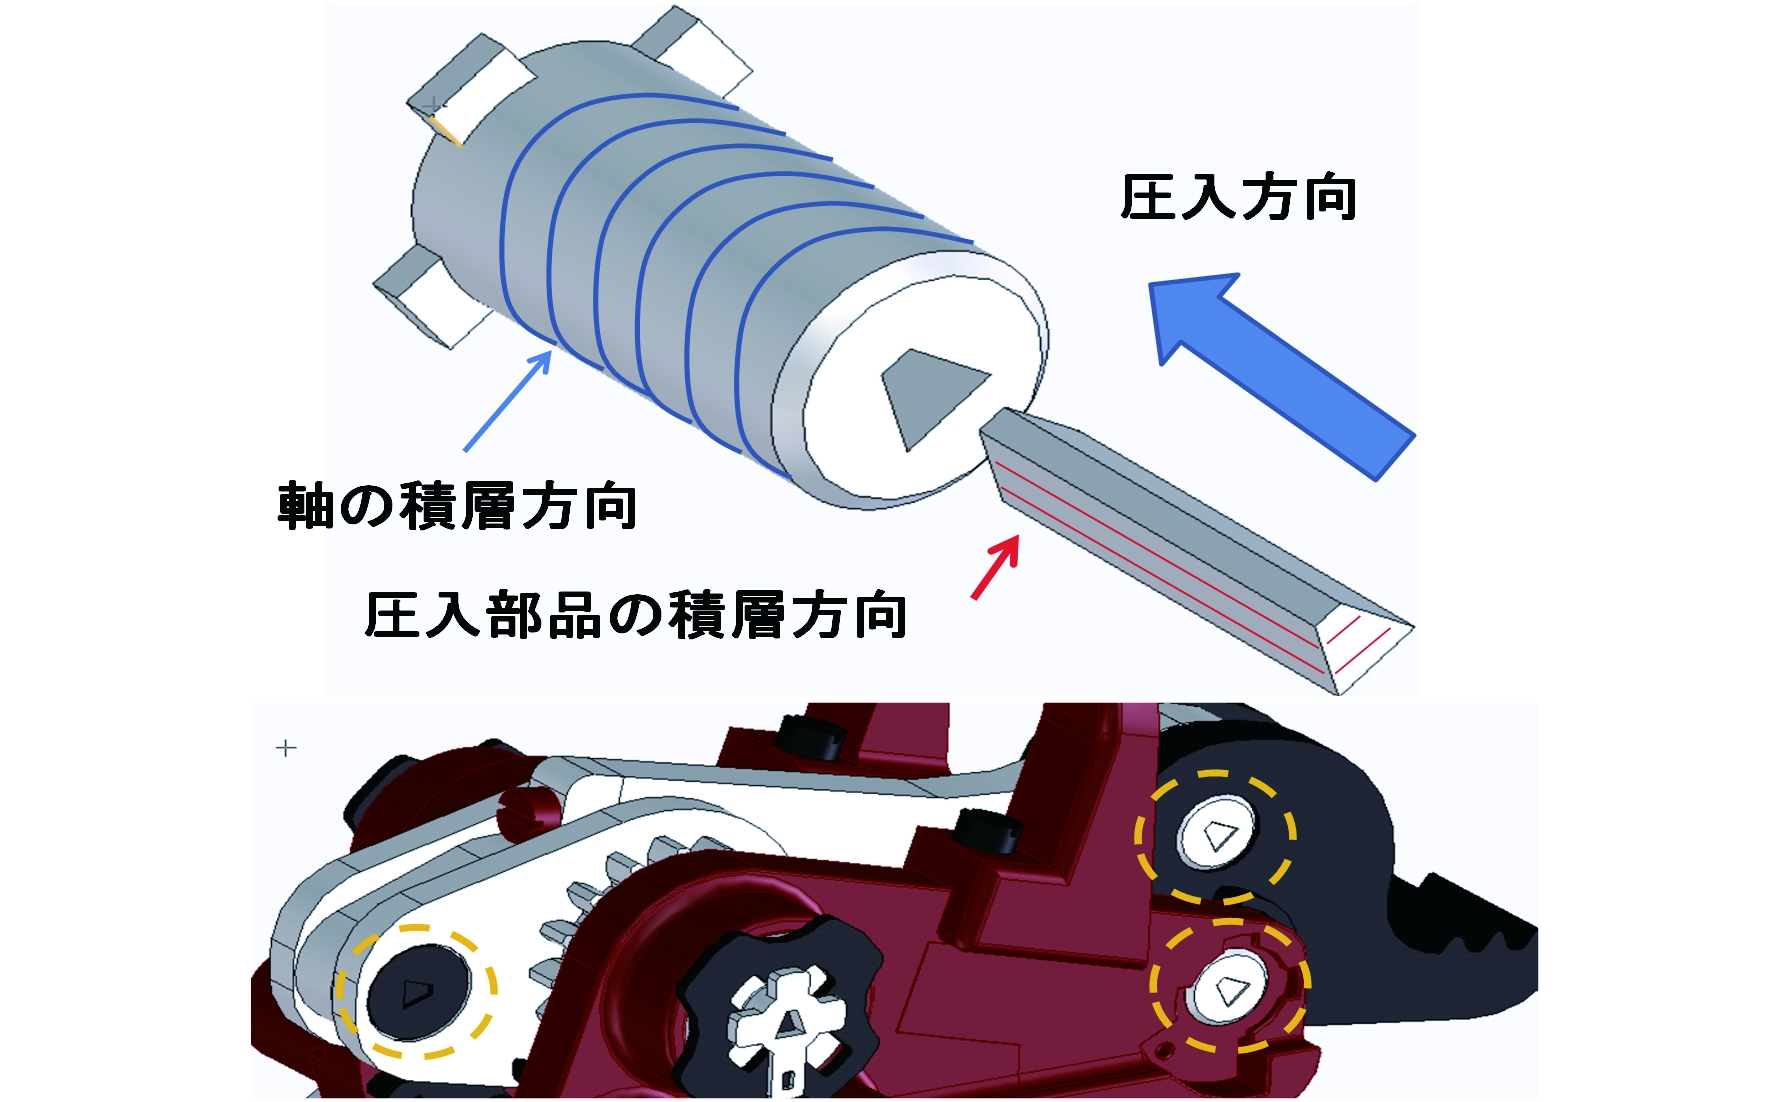
\includegraphics[width=370pt]{fig/fig20_cmyk.jpg}
\caption{積層方向の割れ防止構成}
\label{fig20}
\end{figure}

\clearpage

\section{モータ出力部の削れ防止構成}\label{ux30e2ux30fcux30bfux51faux529bux90e8ux306eux524aux308cux9632ux6b62ux69cbux6210}

ギアドモータ出力部には削れ防止構成を採用して設計しました。
モータ出力部から、3Dプリンタで製作した部品を、アルミ製の駆動伝達部品を介して接続しています。(Fig.\ref{fig19})

\begin{figure}[htbp]
\centering
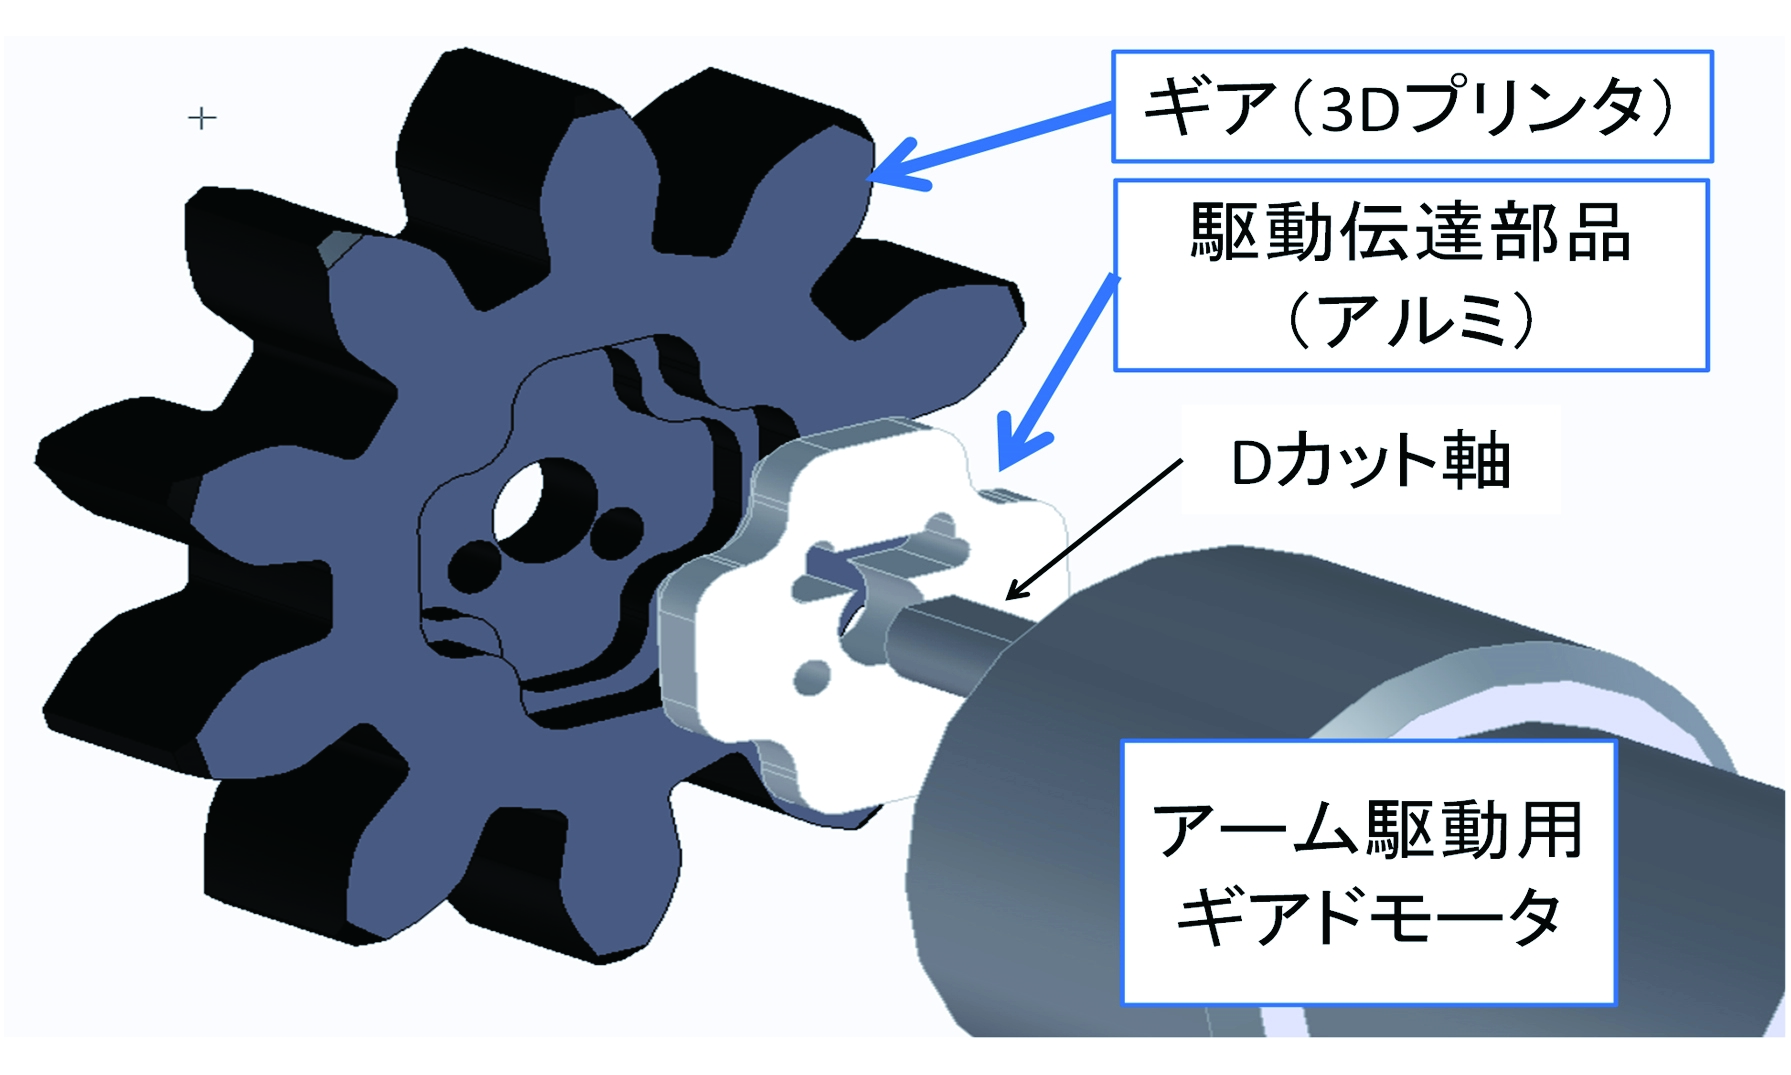
\includegraphics[width=190pt]{fig/fig19_cmyk.jpg}
\caption{モータ出力部の削れ防止構成}
\label{fig19}
\end{figure}

\section{大型部品の作成方法}\label{ux5927ux578bux90e8ux54c1ux306eux4f5cux6210ux65b9ux6cd5}

3Dプリンタのテーブルサイズを超える部品に関しては、分割・結合する必要があります。
本機体では、側面フレームが該当するため、2分割構成としました。
分割した部品同士の結合部に関しては断面形状を六角形とすることで、組立方向以外の方向に力がかかっても外れないようになっています。
また、組立方向を中間フレームに対して傾けることで、側面フレームを中間フレームに結合した後、組立方向に対する外れを防止しています。
(Fig.\ref{fig21})

\begin{figure}[htbp]
\centering
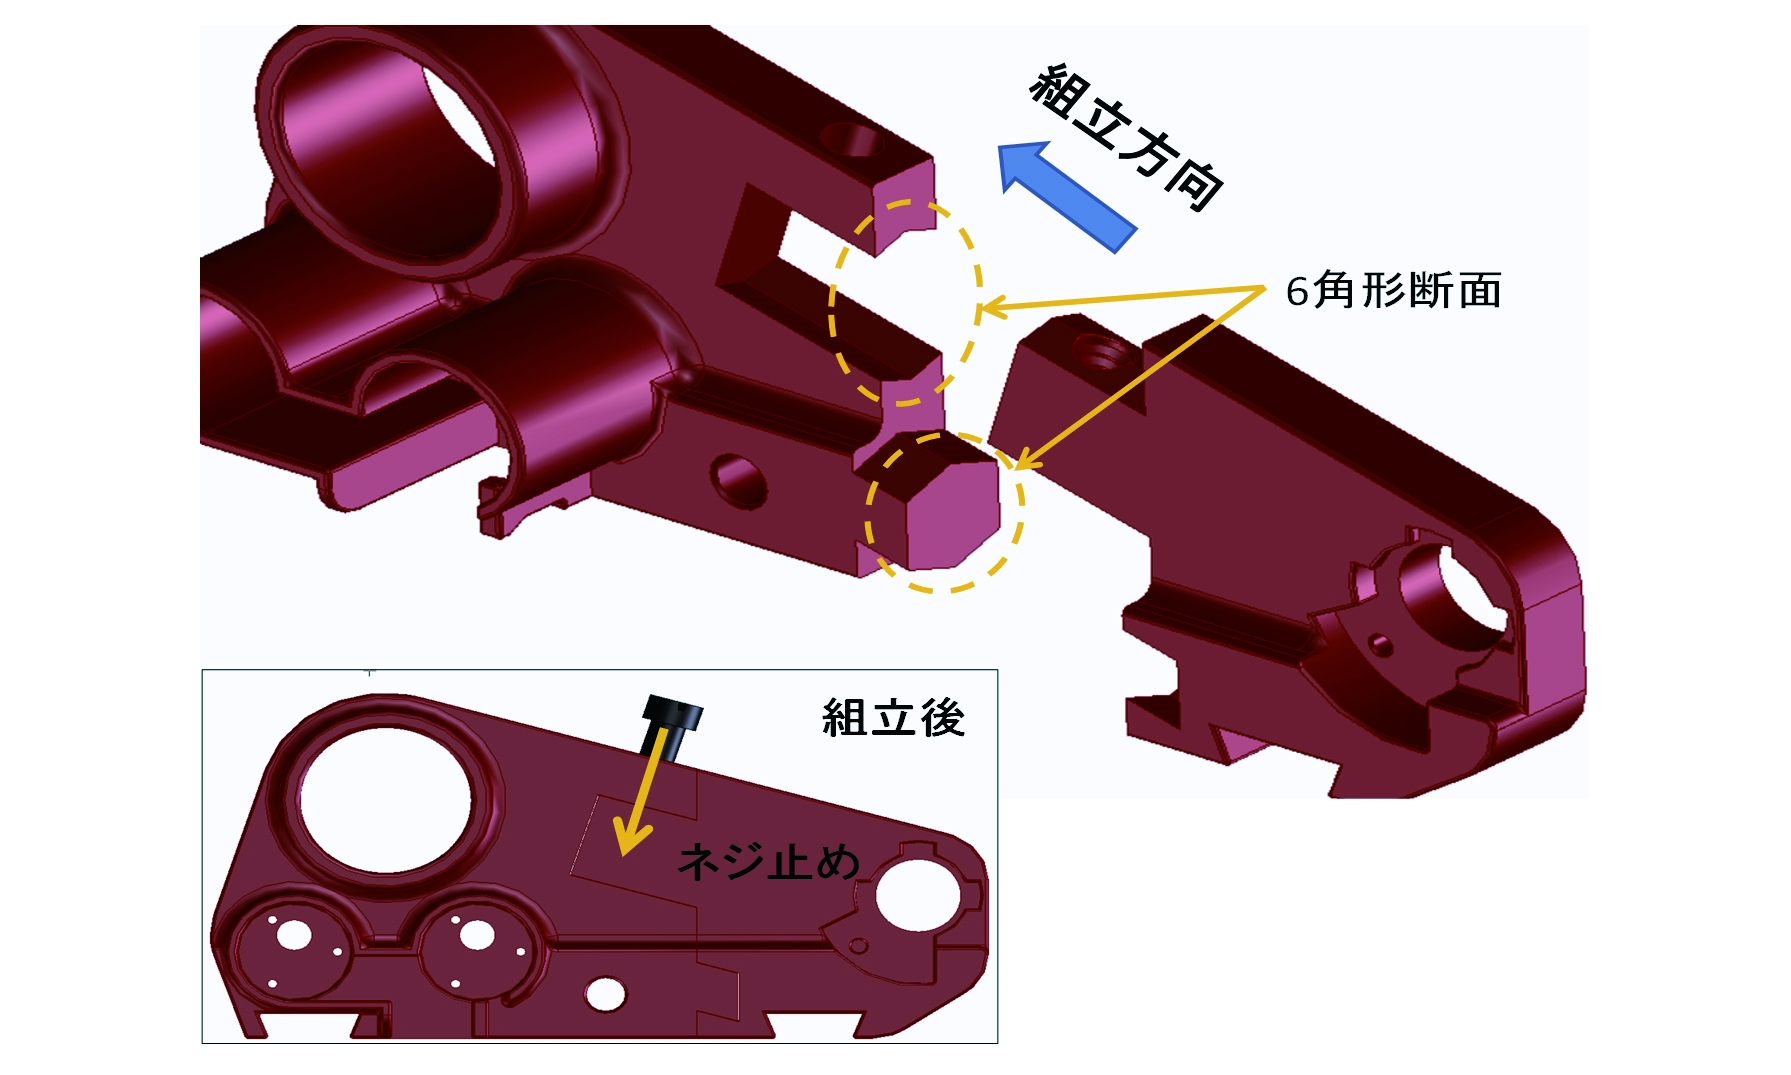
\includegraphics[width=290pt]{fig/fig21_cmyk.jpg}
\caption{大型部品の作成方法}
\label{fig21}
\end{figure}
